\documentclass[sigconf]{acmart}

\usepackage{booktabs} % For formal tables


% Copyright
%\setcopyright{none}
%\setcopyright{acmcopyright}
%\setcopyright{acmlicensed}
%\setcopyright{rightsretained}
%\setcopyright{usgov}
%\setcopyright{usgovmixed}
%\setcopyright{cagov}
%\setcopyright{cagovmixed}


% DOI

%Conference


\begin{document}
\title{Deep Learning Applications on Stock Market Data}

\author{Professor Robert J. Brunner}
\orcid{1234-5678-9012}
\affiliation{%
  \institution{University of Illinois at Urbana-Champaign}
  \institution{Department of Physics} 
  \institution{Department of Astronomy}
  \institution{Department of Statistics}
  \institution{National Center for Supercomputing Applications}
  \city{Urbana} 
  \state{Illinois} 
  \postcode{61801}
}
\email{bigdog@illinois.edu}

\author{Sushma Adari}
\affiliation{%
  \institution{Blue Waters Student Intern}
  \institution{University of Illinois at Urbana-Champaign}
  \institution{Department of Astronomy}
  \institution{Department of Computer Science}
  \city{Urbana} 
  \state{Illinois} 
  \postcode{61801}
}
\email{sadari2@illinois.edu}




% The default list of authors is too long for headers}



\begin{abstract}
This paper aims to outline the different methods of stock market analysis through the use of Neural Networks using the Keras Deep Learning Library for Theano and Tensorflow. The concentration will be on using a type of Recurrent Neural Network (RNN) known as the Long Short Term Memory (LSTM) and the Multilayer Perceptron (MLP) Neural Network. 
\end{abstract}

%
% The code below should be generated by the tool at
% http://dl.acm.org/ccs.cfm
% Please copy and paste the code instead of the example below. 
%

% We no longer use \terms command
%\terms{Theory}

\keywords{Neural Networks, Time-Series Analysis, Stock Market Data, Algorithms,Machine Learning, Deep Learning}

\maketitle

\section{Introduction}

The recent years have shown an increase in interest in Artificial Intelligence (AI) in the science and computing community. A specific subset of AI known as deep learning, which uses neural networks, has gained particular attention as it is a powerful tool that is used across various disciplines including astronomy, physics, finance, mathematics and more. Neural Networks are a computational method based on the way the human brain recognizes and solves problems. The neural network, much like how the brain works, uses a knitted system of simple operational elements and artificial neurons that work in parallel to determine an outcome that is influenced by various pieces of information. The purpose of a neural network is to 'learn' patterns and rules from observational data and replicate the function of groups of neurons and axions within the brain. Neural networks then apply what they have learned on new sets of data in order to identity/predict/classify the new data's characteristics. \cite{kar}Formally a neural network can be defined as follows: 

"Specifically, a neural network is a system composed of many simple processors - fully, locally, or sparsely connected - whose function is determined by the connec- tion topology and strengths. " 
	
    - DARPA Neural Network Study 1988 \cite{DARPANeuralNetworkStudy(U.S.):1988:DNN:576294}
    
    
"Neural Networks are universal function approximators, they are powerful methods for pattern recognition, classification, and forecasting. Neural Networks are less sensitive to noise, chaotic components and, heavy tails better than most other methods."

	-Designing a Neural Network for Forecasting Financial and Economic Time-Series \cite{kaastra1996designing}
    
Neural Networks are a powerful tool that can be applied to a wide range of problems which provide highly accurate solutions however due to their incredible complexity there are many factors that need to be accommodated for before they are suitable for real world applications. Particularly, the field of finance has been neural networks in order to forecast the prices and sales of the market. In finance, neural networks developed out of necessity as the need for rapid, accurate information constantly drives the industry \cite{kar} \cite{kaastra1996designing}.

As such, this paper aims to outline the structure of artificial neural networks along with unique characteristics specific neural networks hold. Next, an overview of the Keras Deep Learning Library will be introduced and its functionality explained with a focus on the Sequential Model. Finally, a brief application of neural networks will be performed on stock market data and the results will be discussed. 

\section{Artificial Neural Networks}\label{sec:ANN}

\subsection{Artificial Neurons}\label{sec:formatting}
\begin{figure}[H]
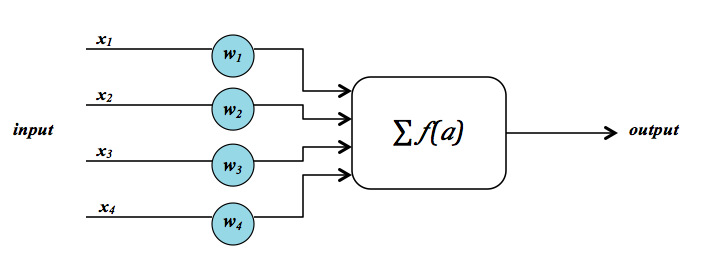
\includegraphics[width=\columnwidth]{ArtificialNeuron}
\captionof{figure}{Artificial Neuron}
\end{figure}
The  artificial neuron aims to replicate the same function of neurons within the brain. Artificial neurons make decisions, based on the importance of the information it receives much like how neurons in the brain sends specific chemical signals based on the chemical signals it receives \cite{kar}. 

 
A simplified functionality of an artificial neuron is describes as follows. An artificial neuron receives N different input parameters, $x_1, x_2... x_N$. Each input is assigned a "weight", $w_1,w_2...w_N$ such that the weight of the input is used to calculate the final output of the neuron. The neurons output is determined by whether or not $ a = \sum_i^N x_i*w_i$ is greater or less than some threshold value defined and sum $a$ is then passed through some activation function such that the $output$ $= f(a)$\cite{kar}

There are various activation functions used to calculate the final output including, Gaussian, sigmoid, hyperbolic tan, binary threshold and more. 
\subsection{Artificial Neural Network}\label{sec:formatting}

A single artificial neuron is not capable of computing the many different boolean functions required in order to solve complex problems. This is solved by connecting the output of some neurons to the input of other neurons, thus creating an artificial neural network. Neural networks are organized through layers, in the figure below, the leftmost most neurons are a part of the input layer and the rightmost neurons are a part of the output layer. The neurons located between the output and input layer is called the hidden layer. Artificial Neural Networks containing more than one hidden layer are referred to as multilayer networks. A neural network that uses outputs from one layer as an input the next layer are known as feedforawrd neural networks in which all of the information passes through the network in a single direction an example of this is a multilayer perceptron neural network (MLP). Neural networks that have connections within the current layer and/or to the previous layer are known as Recurrent Neural Networks (RNN) and are not limited to a linear processing of the information. \cite{kar}
\begin{figure}[H]
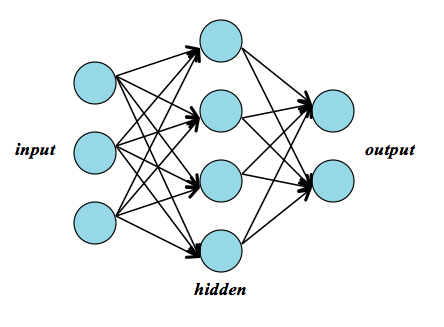
\includegraphics[width=\columnwidth]{neuralnet}
\captionof{figure}{Artificial Neural Network with 1 Hidden Layer}
\end{figure}
\section{Multilayer Perceptron Neural Network}\label{sec:Models}

Multilayer perception neural networks are feedforward networks that involve one or more hidden layers. Each layer is fully connected to the next layer such that each neuron, excluding input neurons, has a non-linear activation function.

The training algorithm used with multilayer perception neural networks is a supervised learning algorithm known as backpropagation. The backpropagation method is a generalization of the Least Mean Squares method which focuses on minimizing the error function. \cite{kar}


\subsection{Backpropagation}\label{sec:cap-num}
Backpropagation is the widley used algorithm for supervised learning with MLP neural networks. The goal of backpropagation is to compute each of the weights of the neural network with respect to an error function (also referred to as a cost function or loss function) through partial derivatives. In the case of backpropagation, the error function refers to the difference between the training input example and the expected output after the training input has been propagated through the network. \cite{nielsen_1970}

In order for backpropagation to be successful there are two assumptions that need to be made about the error function. The first, is that the error function can be written as an average $ E = \frac{1}{n}\sum_{x} E_x$ over all unique training examples x. The reason behind this is so the backpropagation algorithm can compute the partial derivatives for each training example x and then be able to generalize it to the total error function. \cite{nielsen_1970}

The second assumption that needs to be made about the error function is that the error function can be written as a function of outputs from the neural network, such that $E = f(a)$ where $a$ is the outputs of the neural network. \cite{nielsen_1970}

These assumptions allow for the successful use of the backpropagation algorithm. The algorithm itself can be divided into to two phases. A forward pass and the backward pass. 

The forward pass starts with the insertion of a vector $x_N$ into the input layer of the neural network, and the outputs are passed through as forward propagations through the network until the estimated final output of the neural network is generated. \cite{nielsen_1970}

The backward pass begins after the estimated final output of the neural network is generated and are provided with the expected output. Starting at the final layer the expected output is moved back through the neural net where  $\delta_N$, the difference between the estimated output and the expected output is calculated for all hidden and output neurons while simultaneously updating the weights of each in order for the network to provide an estimated output that is closer to the expected value. \cite{nielsen_1970}
\cite{guo2013backpropagation} \cite{hecht1988theory}
The backpropagation algorithm is primarily for feedforward networks, however in RNNs there is a variation of the algorithm known as backpropagation through time which will be covered briefly in the next section.


%% Bug in template?  No space here --foley
\vspace{1.5\baselineskip}
\section{Recurrent Neural Network}
\begin{figure}[H]
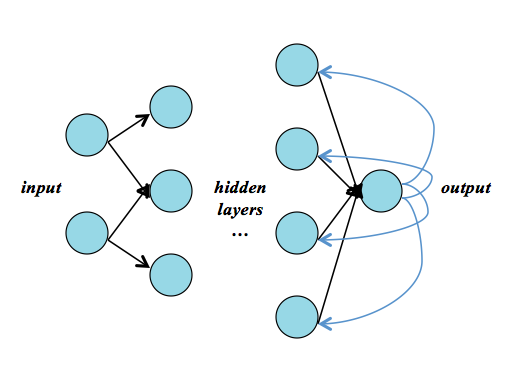
\includegraphics[width=\columnwidth]{RNN}
\captionof{figure}{Recurrent Neural Network}
\end{figure}
Recurrent Neural Networks have become popular amongst scientists as they have become extremely successful when applied to various research subjects.
Unlike MLP neural netowrks, RNNs are not feedforward and can contain connections within the current layer and to previous layers. Within a traditional feedforward network the input vector, the output vector and the amount of computational steps is a fixed value. However, within a recurrent neural network, computation can be computed on sequences of the input vector or output vector. As such recurrent neural networks are more powerful than a feedforward network. \cite{nicholson} \cite{olah} In a feedforward neural network the output vector is influenced by the input vector, in a RNN the network is influenced by not only the input vector but also all of the history of previous inputs. Like MLP neural networks, RNNs also rely on backpropagation but they use a variation known as backpropagation through time (BPTT), the key difference between the standard backpropagation algorithm and BPTT is that gradients are summed up over the layers since RNNs are not feedforward and can have dependencies on the current layer and/ previous layers. BPTT ensures that all changes in weights are accounted for. \cite{nicholson} \cite{olah}

One of the advantages of using an RNN is the ability to look back to previous information and use it in the current task. RNNS are capable of gathering relevant information however only to a certain limit. If the information the RNN needs to compute is relatively near the current, the space needed to hold that information is also small. In cases, where the RNN needs to reach much farther back to get information, the RNN, in practice, is no longer able to learn to connect to the previous relevant information. \cite{olah}

This is known as the vanishing gradient problem. In a recurrent neural network information passes through the neural net undergoes multiple stages of multiplication as a result when gradients are computed the values become too small for the network to learn on. \cite{nicholson}

Due to the vanishing gradient problem, a variation of the RNN known as Long Short Term Memory (LSTM) was developed so that neural nets can learn long term dependencies. 
\subsection{Long Short Term Memory}

LSTMs are a special variation of the RNN designed to avoid the long-term dependency problem, by remembering long sequences of information without having to learn them.

LSTMs are built with memory gates with a unique feature known as a gated cell which regulates what information can be stored, written, or read through gate openings and closings. The gates are made of a sigmoid neural net layer which outputs values between zero and one through pointwise multiplication operations, indicating how much information should be passed through. Zero corresponding to let no information pass and one corresponding to let all the information pass. \cite{nicholson} \cite{olah}
\begin{figure}[H]
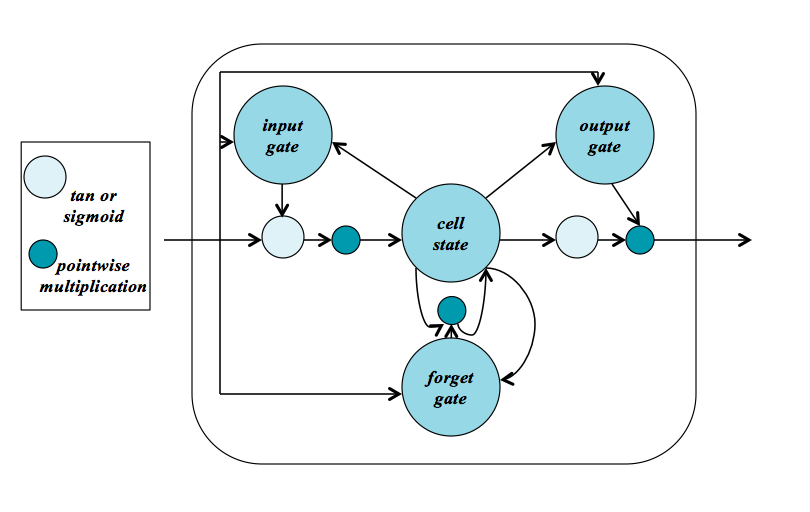
\includegraphics[width=\columnwidth]{LSTMCell}
\captionof{figure}{Long Short Term Memory Cell \cite{DBLP:journals/corr/GreffSKSS15}}
\end{figure}
In order to build a successful LSTM, a combination of gates are used to determine what information is relevant to the current problem. First within the forget gate layer, the LSTM neural network decides whether or not to keep the information in the current cell state. This layer computes a value between zero and one in order to determine how much information should be remembered in the current state. The next layer is the input gate layer which determines which new information, if at all, should be included in the cell state, once again a value between zero and one is computed to determine the extent of new information that should be remembered. Finally, the output gate layer determines which information in the current state should be outputted. \cite{nicholson}\cite{olah}

LSTMs are used far more frequently than the general recurrent neural network since they account for the vanishing gradient problem and are capable of solving a larger variety of problems.
\section{Keras}\label{models}

"Keras is a high-level neural networks API, written in Python and capable of running on top of either TensorFlow or Theano. It was developed with a focus on enabling fast experimentation. Being able to go from idea to result with the least possible delay is key to doing good research."

-Keras Documentation \cite{chollet2015keras}

The implementation of the MLP neural network and LSTM neural network for predicting trends in stock market data was completed through Keras Deep Learning Library. In this section, a brief outline of the Keras Sequential model will be discussed followed by an brief explanation of the implementation of the MLP and LSTM neural networks and the factors that were taken into consideration upon building them. 

The sequential model in Keras is a linear stack of layers. \cite{chollet2015keras} First construct a Sequential model and add the layers of computation in the desired order. The first add will correspond to the input layer in which the input dimension should be defined, this is also where the type of network can be be define such as LSTM. In Keras, fully connected layers are defined by the Dense class in which the first parameter is the number of neurons in the layer, the second is the initialization method, and the third is the activation method. Often, the hidden layers and the input layer use the rectifier activation function in order to have better performance and the output layer activation function is chosen based on what format the intended predictions should take. A full list of the initializations and activations can be found in the Keras Documentation. \cite{2017} \cite{brownlee_2017_0}

After defining the layers of the neural network using the Sequential model, the learning process of the model will be configured using the compile method. Compilation is mandatory as Keras will determine the most effective way to represent the neural network for training. Keras finds the best representation of the neural network such that it runs on the appropriate hardware such as CPUs and GPUs. In order to compile the model, a number of variables need to be defined that should be specific to training the network. An error function, defined as loss function on the documentation, and an optimizer should be defined along side any of the other optional metrics. A full list of available optimizers and loss functions can be found in Keras Documentation. \cite{2017} \cite{brownlee_2017_0}

The next step is to train the network with the training set using the fit function. The fit method will run through the dataset in a fixed number of iterations known as epochs defined by the nb\_epoch argument. Each epoch can be further divided into input-output pairs defined by the batches argument which defines the number of evaluations that occur before the weights in the network are updated. \cite{2017} \cite{brownlee_2017_0}

The next step is the evaluate the model. Performance can be either evaluated on the same dataset that training was done on or on another dataset. Performing evaluation on the same dataset does not provide any information on how well the algorithm performs on new data, therefore a dataset that the model has not seen before will better represent how accurate the model performs with new data. the evaluate function takes in the same input and output parameters passed as when the fit function was called. A list of evaluation metric will be returned after the model computes the loss across all the evaluations as well as any additional metrics that were defined with the model. \cite{2017} \cite{brownlee_2017_0}

Finally, after determining that the model is accurate it can be used for prediction using the predict function. This is simply done by calling predict on the model using a new input set of data and the result will be returned as defined by the output layer of the network. \cite{2017} \cite{brownlee_2017_0}

This is the general outline to be followed when creating a Keras Sequential model, often defining the layers and the parameters to include are found through trial and error as there is no completely accurate way of defining the what parameters should be chosen when building the model. 

\section{Stock Market Data Applications}\label{data}

This section will describe the dataset, the preprocessing steps taken to use the dataset, and finally there will be a brief outline of the Keras MLP and LSTM neural network implementation. 

The aim of the neural networks in each case is to accurately predict the midquote value of the stock by setting a 'look back' value which is the amount of time steps  for the neural network to account for when predicting the midquote values at the next time-steps.

\subsection{Data Format}\label{sec:data}
The dataset consists of minute level stock data spanned from the years 1993 to 2010, the dataset is organized in five columns named: PERMNO, SYMBOL, DATE, itime, and mquote. PERMNO corresponds to a unique identification number of each stock, SYMBOL corresponds to the stock's ticker symbol, DATE is the date in Julian date format, itime is the time between 9:30:00 AM to 4:30:00 PM and mquote corresponds to midquote price of the stock at the specified date and time. 

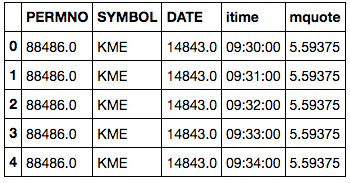
\includegraphics[width=\columnwidth]{datatable}
\captionof{figure}{Dataframe of Stock KME}

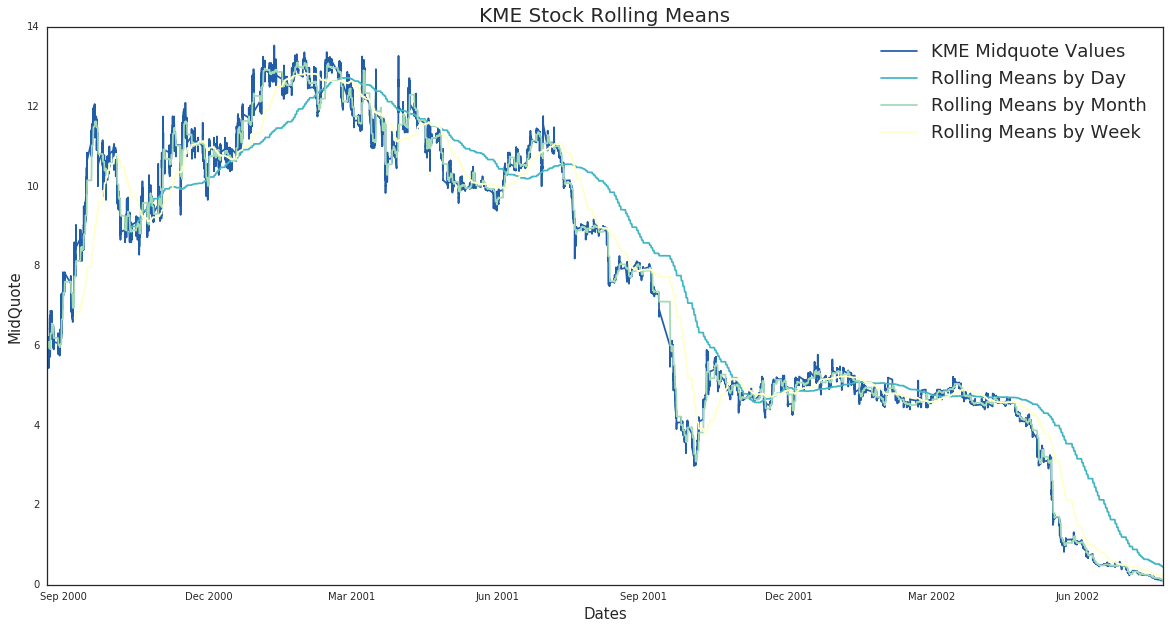
\includegraphics[width=\columnwidth]{RollingM}
\captionof{figure}{Time-Series Plot of Stock KME with Rolling Means}

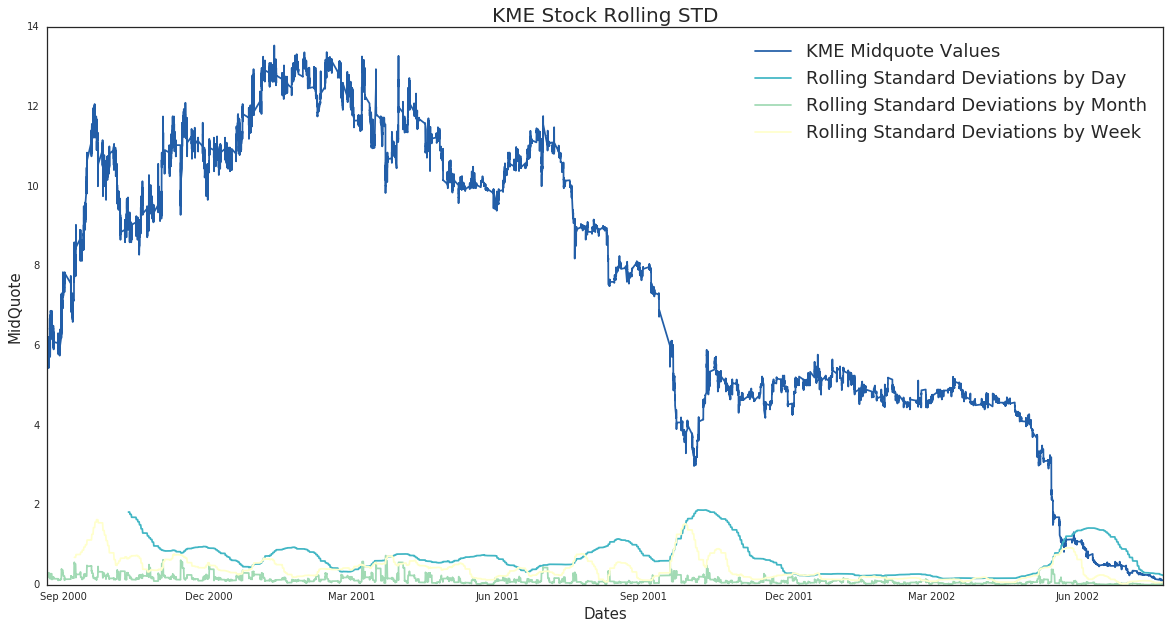
\includegraphics[width=\columnwidth]{RollingS}
\captionof{figure}{Time-Series Plot of Stock KME with Rolling Standard Deviations}
\subsection{Data Preprocessing}\label{sec:data}


The data was initially received in the format of 13671 sas7bdat files and was converted into csv files using the sas7bdat.py module. After all the files were converted, a brief run through of them was completed and empty csv files within the dataset were discarded. With the csv files, a sqlite database was constructed where each table within the database corresponds to an individual stock. 

\subsection{Keras Multilayer Perceptron Neural Network}\label{sec:data}

First, the dataset was split into train and testing dataset. In this instance the dataset is split as follows: 67\% train and 33\% test. Three MLP Neural Networks were constructed $MLP_1$, $MLP_2$, $MLP_3$. $MLP_1$ containing one hidden layer, $MLP_2$ containing two, and $MLP_3$ containing three. Each input layer contained sixteen neurons and initially computed with a look-back of 10. $MLP_1$ single hidden layer contained 8 neurons with the output layer containing one. $MLP_2$ first hidden layer contained 8 neurons and the second four with the output layer containing one. $MLP_3$ fist hidden layer contained 8 neurons, second 4, third 2 and output containing one. The activation function selected for each layer was rectifier activation function. \cite{brownlee_2017_1}

The Rectifier Linear Function sets the neurons threshold to zero and has an advantage over the hyperbolic tan (tanh) and sigmoid activation functions since unlike tanh and sigmoid operations it does not contain many computationally expensive operations. In addition, it is known  to have a much shorter training time. 

The loss function used for each MLP is the mean-squared-loss and the optimization function defined is 'Adam'.

Each MLP was compiled, evaluated and predicted on both the train and the test. The results are shown in the graphs below.
\begin{figure}[H]
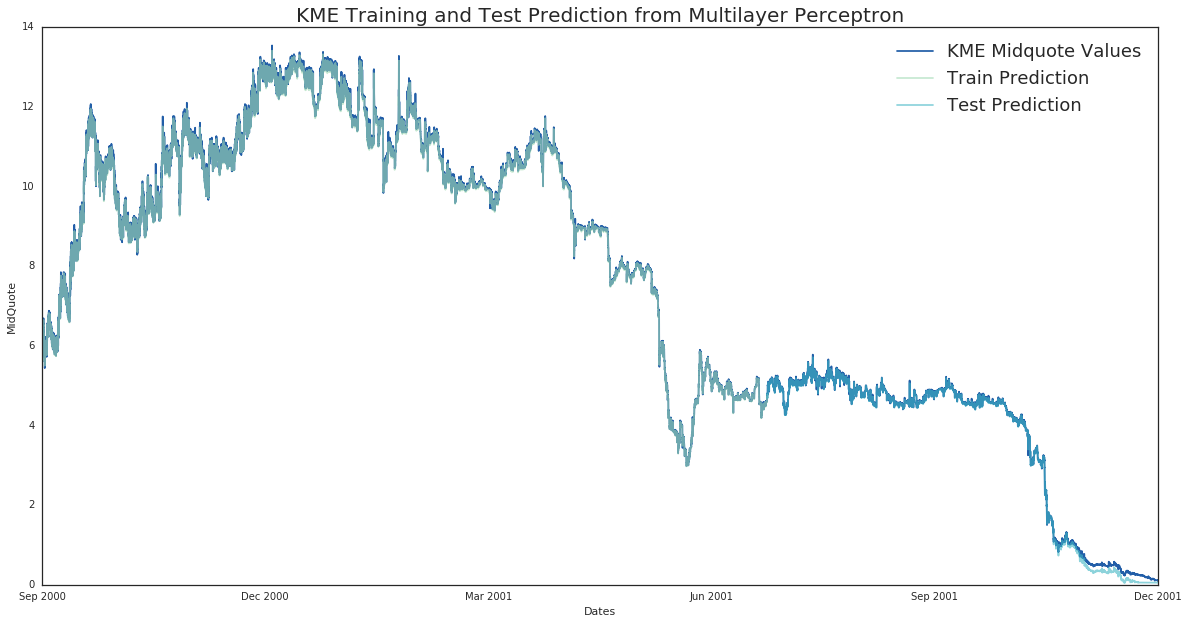
\includegraphics[width=\columnwidth]{hidden1lb10}
\captionof{figure}{KME Stock Prediction with MLP 1 Hidden Layer and  Look Back = 10 \\ Train Score: 0.00587689609176 \\
Test Score: 0.00059857688262 \\
Mean Squared Error of Training =  0.0111476820422 \\
Mean Squared Error of Test =  0.0007153639125
}
\end{figure}
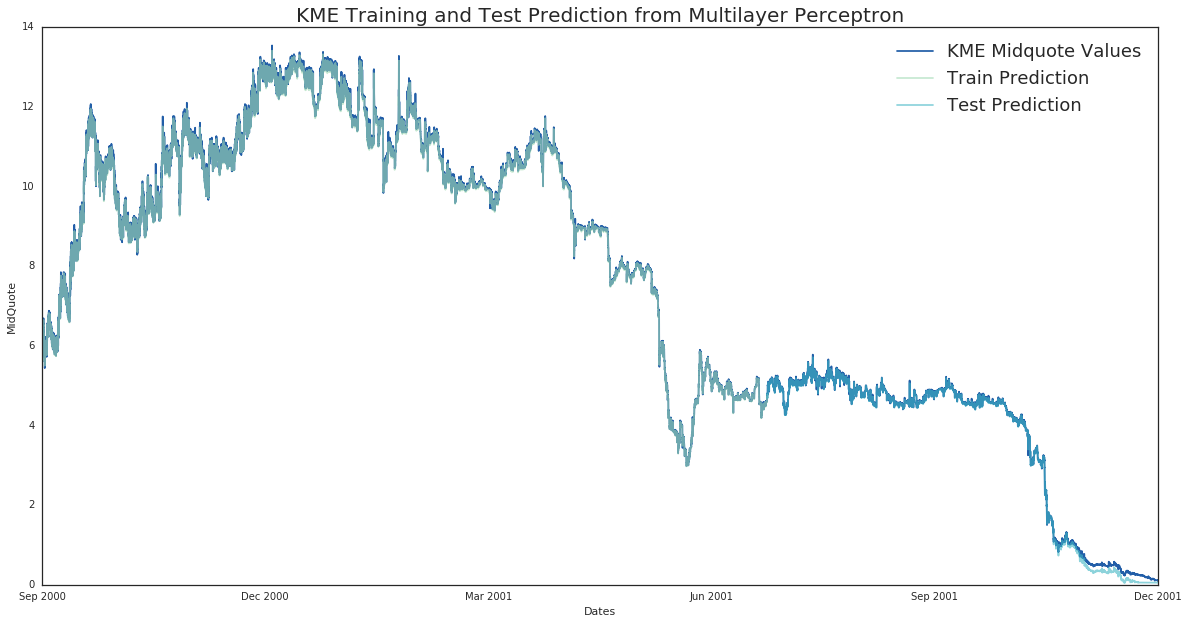
\includegraphics[width=\columnwidth]{hidden2lb10}
\captionof{figure}{KME Stock Prediction with MLP 2 Hidden Layers and  Look Back = 10 \\ Train Score: 0.00440365362902 \\
Test Score: 0.00563585469968  \\
Mean Squared Error of Training =  0.010273679736 \\
Mean Squared Error of Test =  0.00575278136196
}
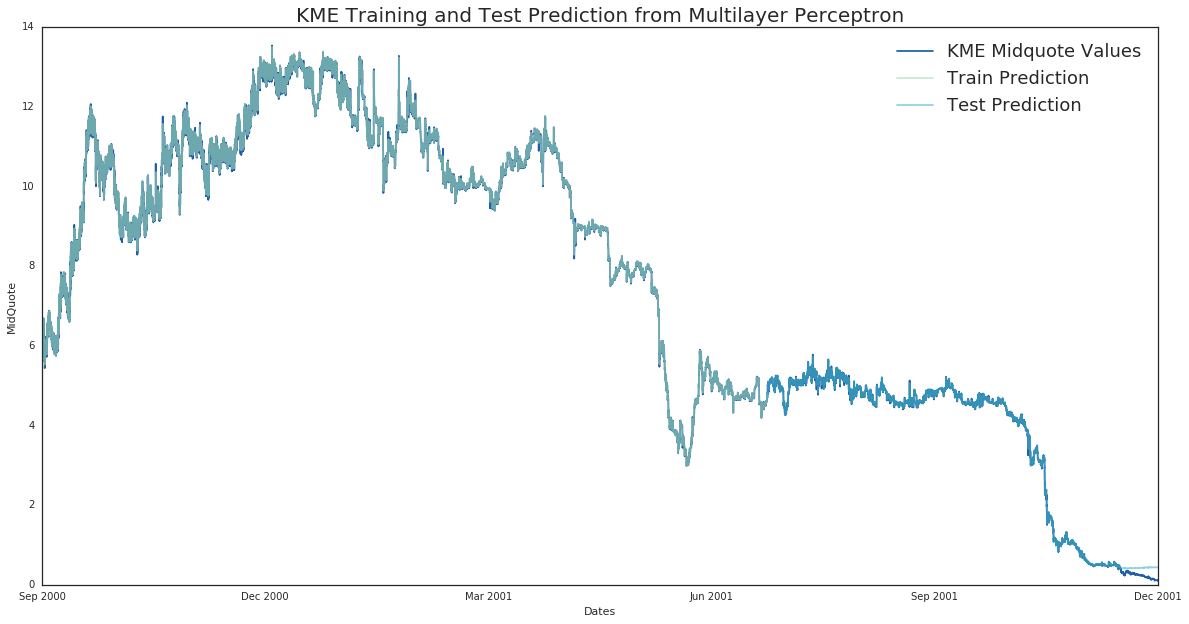
\includegraphics[width=\columnwidth]{hidden3lb10}
\captionof{figure}{KME Stock Prediction with MLP 3 Hidden Layers and  Look Back = 10 \\ Train Score: 0.00320127937628 \\
Test Score: 0.0043091359383 \\
Mean Squared Error of Training =  0.00896512464735 \\
Mean Squared Error of Test =  0.00443209335173 
}
The results are incredibly accurate as both the training and testing mean squared errors are very low. 
In order to further explore the application of MLPs on the data, $MLP_3$ was run with  look-back times 100 and 1000 times steps in order to gauge how well the neural network can predict the right midquote value when increasing the amount of previous times steps the neural networks has to use to predict the next values. 
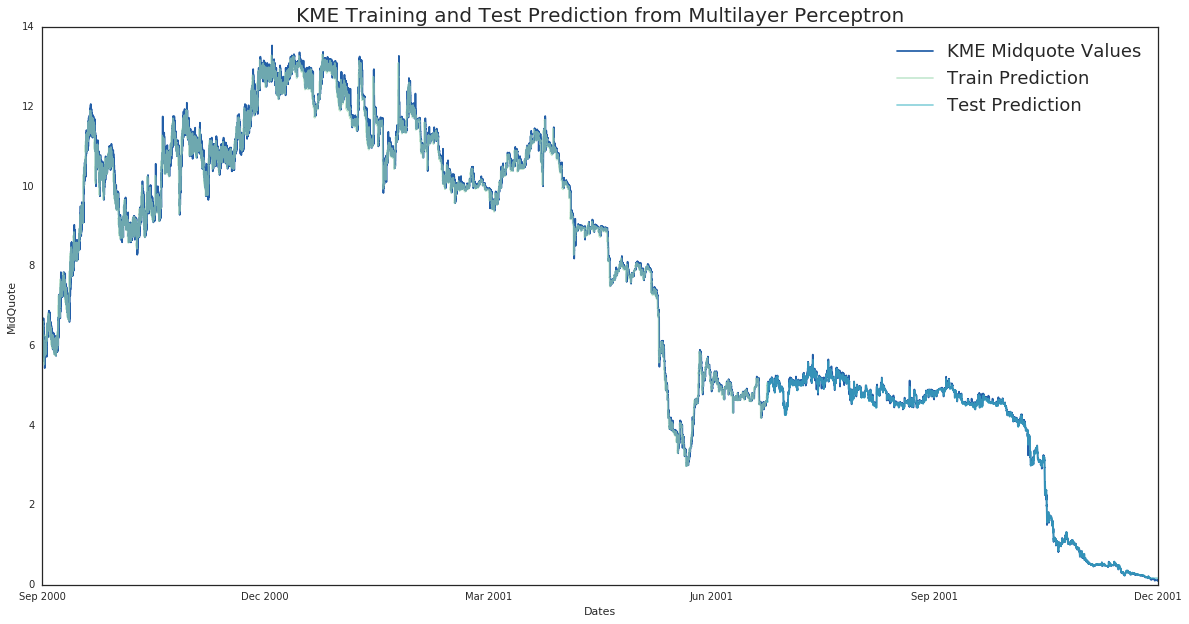
\includegraphics[width=\columnwidth]{hidden3lb100}
\captionof{figure}{KME Stock Prediction with MLP 3 Hidden Layers and  Look Back = 100 \\ Train Score: 0.00467338790759 \\
Test Score: 0.000394619438351\\
Mean Squared Error of Training =  0.0424847103314\\
Mean Squared Error of Test =  0.000500693180888
}
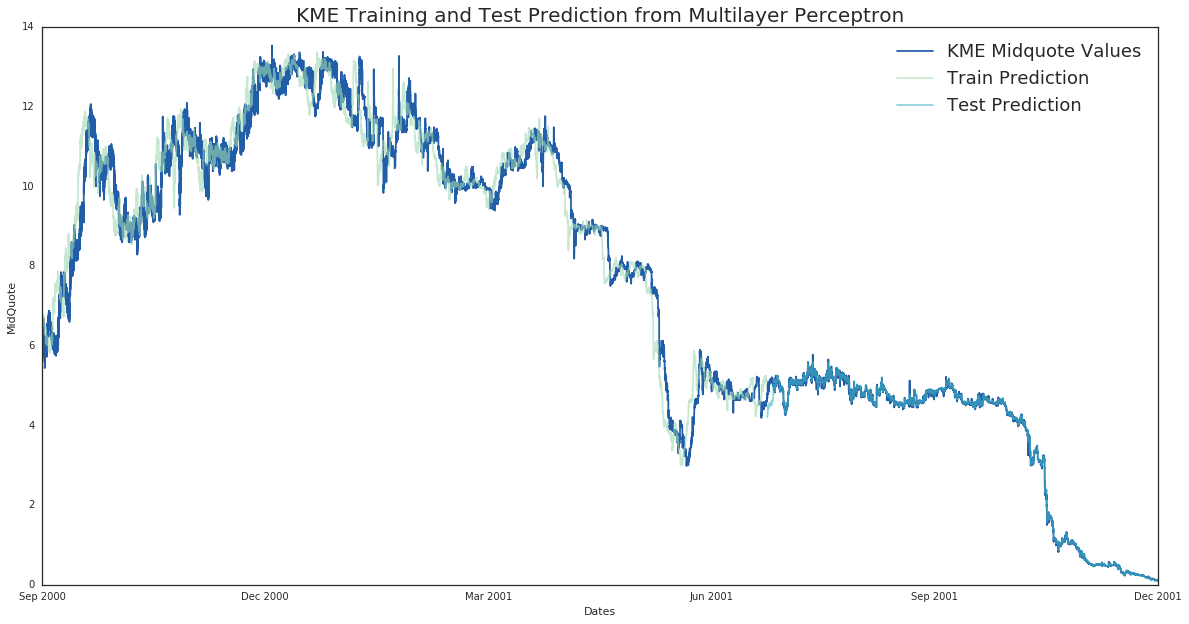
\includegraphics[width=\columnwidth]{hidden3lb1000}
\captionof{figure}{KME Stock Prediction with MLP 3 Hidden Layers and  Look Back = 1000 \\ Train Score: 0.00677010296607 \\
Test Score: 0.000748885668976\\
Mean Squared Error of Training =  0.363470126085 \\
Mean Squared Error of Test =  0.000839856101171
}
Increasing the amount of time-steps did not deter the accuracy of the neural network much and still provided accurate results. 

\subsection{Keras Long Short Term Neural Network}\label{sec:data}

In addition to applying a MLP neural network on the data a Long Short Term Memory neural network was applied as well. 

Unlike when running the MLPs on the data, for the lstm models the data was normalized using SciKit learn's MinMaxScaler function, so it did not encounter errors when passing through the sigmoid activation functions in the output layer. The LSTM neural network was defined again with 3 hidden layers, each hidden layer including the input layer uses the rectifier activation function and the output layer uses the sigmoid activation function and the Adam optimizer was used for each layer. \cite{brownlee_2017_0}
After compiling, evaluating and predicting, the predicted results were transformed back from normalized values using Scikits inverse transform. 

The LSTM neural network is run on a look-back of 10, 100, and 1000. The results are shown below:

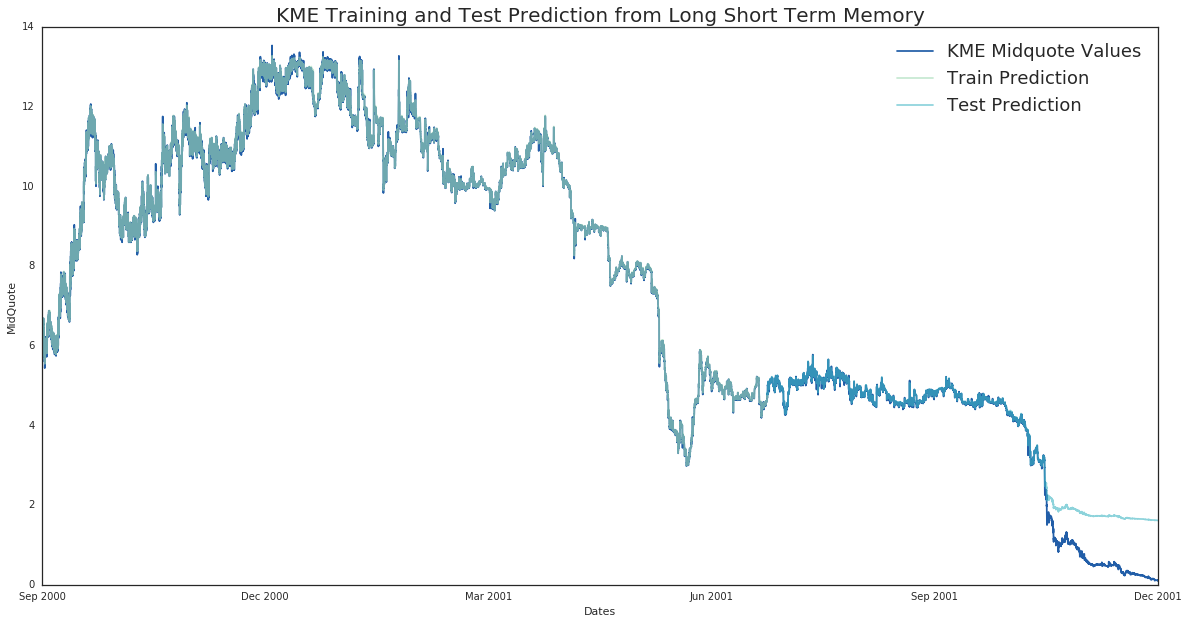
\includegraphics[width=\columnwidth]{lstmhidden3}
\captionof{figure}{KME Stock Prediction with LSTM 3 Hidden Layers and  Look Back = 10 \\ Train Score: 1.85937403344e-05 \\
Test Score: 0.00221193562789\\
Mean Squared Error of Training =  0.00931988605579 \\
Mean Squared Error of Test =  0.398898080738
}
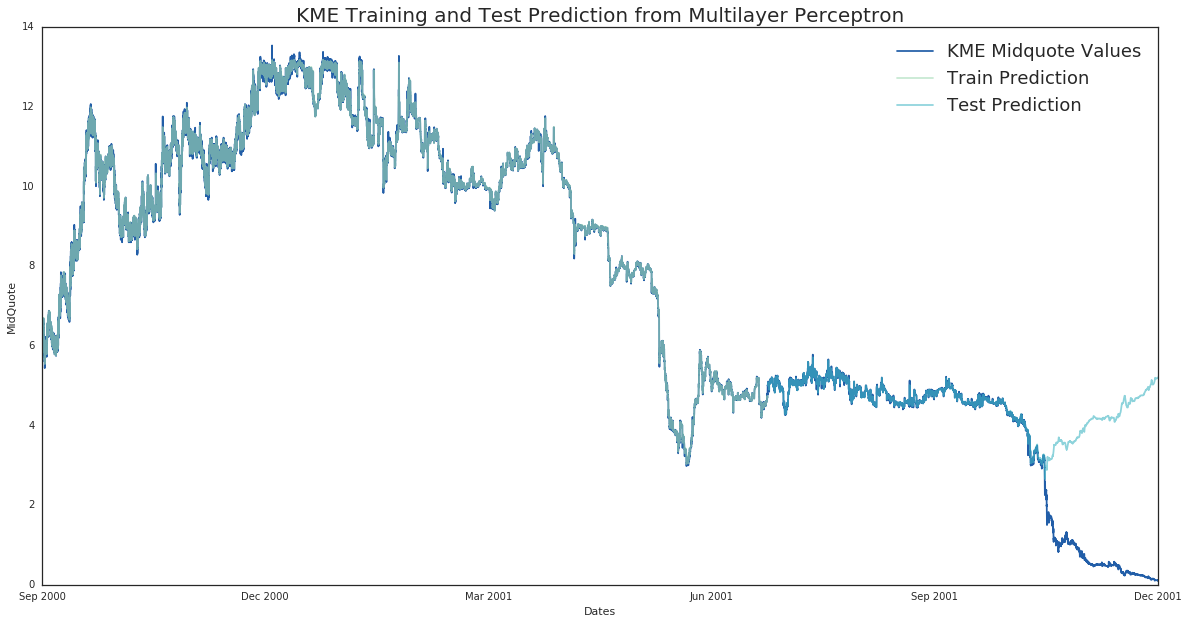
\includegraphics[width=\columnwidth]{lstmhidden3lookback100}
\captionof{figure}{KME Stock Prediction with LSTM 3 Hidden Layers and  Look Back = 100 \\ Train Score: 1.89597180758e-05 \\
Test Score: 0.0211583475203\\
Mean Squared Error of Training =  0.0433826336754 \\
Mean Squared Error of Test =  3.81435184278
}
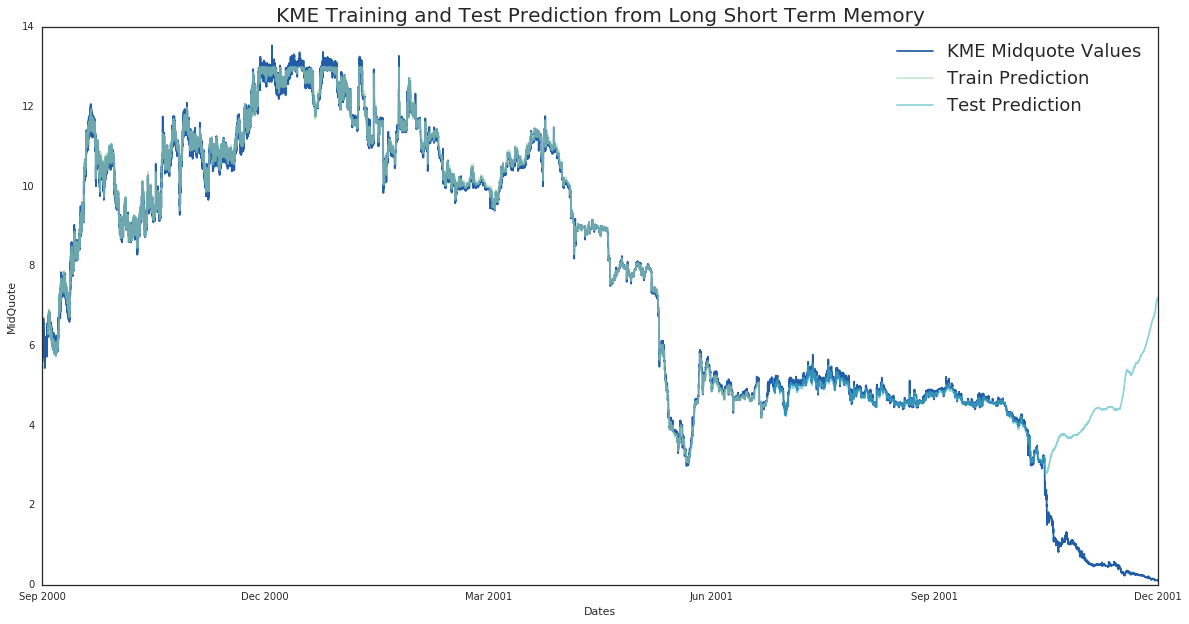
\includegraphics[width=\columnwidth]{lstmlb1000}
\captionof{figure}{KME Stock Prediction with LSTM 3 Hidden Layers and  Look Back = 1000 \\ Train Score: 4.2847528867e-05 \\
Test Score: 0.0281624968257\\
Mean Squared Error of Training =  0.369410562767 \\
Mean Squared Error of Test =  5.07693484985
}
Even in the case of LSTMs, the neural network performs well, although in the test data set the fit was a little less accurate when in comparison to the MLP neural network's outputs. However, this can be easily be accounted for by creating further variations and specifications to the LSTM to ensure that it is more suited to the data.
\subsection{Further Applications}\label{sec:data}

Outside of basic midquote value predictions, there are many other applications that neural networks on stock data can be applied to. One particular area of interest is using correlations within specific market sectors. By finding two stocks that have a strong correlation between the percent change in midquote values, a neural network can be trained on one and then used to predict the other. This application may especially be useful in determining underlying relationships within the market that are not easily apparent at first glance.  

\section{Conclusion}

Neural Networks are powerful tools capable of accomplishing great feats with high accuracy. By replicating the decision making process found within the human brain, neural networks are able learn of datasets to produce precise predictions and classifications. In the case of predicting the stock market medium, there is a strong potential in producing  neural networks to learn off of the stock market data. Even simple MLPs and LSTMs are able to produce significant results with incredible accuracy. Applying these neural networks to much larger datasets will help to provide more information on how the financial markets work and can even be used to detect underlying features within the market that are not immediately present. Neural networks are a powerful tool that can be used effectively to gather more information on the stock market medium. 

\section{Acknowledgements}

Sushma Adari and Professor Robert J. Brunner would like to thank Shodor Organization and the National Center for Supercomputing Applications for the generous funding and resources in order to work on and develop this project. 


\bibliographystyle{ACM-Reference-Format}
\bibliography{sigproc} 

\end{document}
